\documentclass{article}

\title{Application of \texttt{Ar-Ar\_Redux} to \textit{WiscAr}
  Noblesse data.}  \author{Pieter Vermeesch\\ London Geochronology
  Centre\\ University College London}

\usepackage{natbib,fullpage,graphicx,caption}

\makeatletter
\def\bbordermatrix#1{\begingroup \m@th
  \@tempdima 4.75\p@
  \setbox\z@\vbox{%
    \def\cr{\crcr\noalign{\kern2\p@\global\let\cr\endline}}%
    \ialign{$##$\hfil\kern2\p@\kern\@tempdima&\thinspace\hfil$##$\hfil
      &&\quad\hfil$##$\hfil\crcr
      \omit\strut\hfil\crcr\noalign{\kern-\baselineskip}%
      #1\crcr\omit\strut\cr}}%
  \setbox\tw@\vbox{\unvcopy\z@\global\setbox\@ne\lastbox}%
  \setbox\tw@\hbox{\unhbox\@ne\unskip\global\setbox\@ne\lastbox}%
  \setbox\tw@\hbox{$\kern\wd\@ne\kern-\@tempdima\left[\kern-\wd\@ne
    \global\setbox\@ne\vbox{\box\@ne\kern2\p@}%
    \vcenter{\kern-\ht\@ne\unvbox\z@\kern-\baselineskip}\,\right]$}%
  \null\;\vbox{\kern\ht\@ne\box\tw@}\endgroup}
\makeatother

\begin{document}

\maketitle

The Noblesse data reduction workflow will be illustrated with a
hypothetical dataset that consists of two blanks ($B1$ and $B2$), two
standard gas shots ($G1$ and $G2$) and three `samples' ($S1$, $S2$ and
$S3$). The latter could either be real samples, J-standards, or
interference monitors. Suppose that these seven runs take place in the
following order:

\[
B1 - G1 - S1 - S2 - G2 - S3 - B2
\]

\section{Read the time-resolved data}

The five Argon isotopes are measured in two `hops', referred to as
`101' and `102' below. In the first hop,
\textsuperscript{36,37,39,40}Ar are measured on the four ion counters
(referred to as $IC0$ through $IC3$).  \textsuperscript{38}Ar is
measured on the axial Faraday cup and is discarded.  In the second
hop, \textsuperscript{36,38,39}Ar are measured on the ion counters and
\textsuperscript{37}Ar is measured on the Faraday cup and discarded.
These time resolved mass spectrometer signals can be read into two
matrices:

\begin{equation}
  X(101) = \left[
    \begin{array}{ccccccc}
      X^{101}_{B1} & X^{101}_{G1} & X^{101}_{S1} &
      X^{101}_{S2} & X^{101}_{G2} & X^{101}_{S3} & X^{101}_{B2}
    \end{array}
    \right]
\end{equation}

\noindent and

\begin{equation}
  X(102) = \left[
    \begin{array}{ccccccc}
      X^{102}_{B1} & X^{102}_{G1} & X^{102}_{S1} &
      X^{102}_{S2} & X^{102}_{G2} & X^{102}_{S3} & X^{102}_{B2}
    \end{array}
    \right]
\end{equation}

\noindent where

\begin{equation}
  X^{101}_{x} =
  \bbordermatrix{
    ~   & IC(0) & IC(1) & IC(2) & IC(3) \cr
    t_1 & 40(1) & 39(1) & 37(1) & 36(1) \cr
    t_2 & 40(2) & 39(2) & 37(2) & 36(2) \cr
    \vdots & \vdots & \vdots & \vdots & \vdots \cr
    t_n & 40(n) & 39(n) & 37(n) & 36(n)
  }
\end{equation}

\noindent and

\begin{equation}
  X^{102}_{x} =
  \bbordermatrix{
    ~   & IC(0) & IC(1) & IC(2) \cr
    t_1 & 39(1) & 38(1) & 36(1) \cr
    t_2 & 39(2) & 38(2) & 36(2) \cr
    \vdots & \vdots & \vdots & \vdots \cr
    t_n & 39(n) & 38(n) & 36(n)
  }
\end{equation}

\noindent for $x \in \{B1, G1, S1, S2, G2, G3, B2\}$.

\section{Blank correction}

Assuming that all measurements are identically set up, the blank
correction is most easily applied to the time-resolved data.  So blank
correction occurs before and not after regression to `time zero':

\begin{equation}
  B(101) = \left[
    \begin{array}{cc|ccc}
      B^{101}_{G1}(B1) & B^{101}_{S1}(B1) & B^{101}_{S2}(B2) &
      B^{101}_{G2}(B2) & B^{101}_{S3}(B2)
    \end{array}
    \right]
\end{equation}

\noindent and

\begin{equation}
  B(102) = \left[
    \begin{array}{cc|ccc}
      B^{102}_{G1}(B1) & B^{102}_{S1}(B1) & B^{102}_{S2}(B2) &
      B^{102}_{G2}(B2) & B^{102}_{S3}(B2)
    \end{array}
    \right]
\end{equation}

\noindent where

\begin{equation}
  B^{y}_{x}(Bz) = X^y_x - X^y_{Bz}
\end{equation}

\noindent for $x \in \{G1, S1, S2, G2, G3\}$, $y \in \{101, 102\}$,
and $z \in \{1, 2\}$.

\section{Form log-ratios}

Let $l36(i), l37(i), l38(i), l39(i)$ and $l40(i)$ be the logarithms of
the $i$\textsuperscript{th} time-resolved and blank-corrected
\textsuperscript{36,37,38,39,40}Ar measurement. Then form

\begin{equation}
  L(y) = \left[
    \begin{array}{cc|ccc}
      L^{y}_{G1} & L^{y}_{S1} & L^{y}_{S2} & L^{y}_{G2} & L^{y}_{S3}
    \end{array}
    \right]
\end{equation}

\noindent where $y \in \{101, 102\}$ and

\begin{equation}
  L^{101}_{x} =
  \bbordermatrix{
    ~   & l(0/9) & l(7/9) & l(6/9) \cr
    t_1 & l40(1)-l39(1) & l37(1)-l39(1) & l36(1)-l39(1) \cr
    t_2 & l40(2)-l39(2) & l37(2)-l39(2) & l36(2)-l39(2) \cr
    \vdots & \vdots & \vdots & \vdots \cr
    t_n & l40(n)-l39(n) & l37(n)-l39(n) & l36(n)-l39(n)
  }
\end{equation}

\noindent and

\begin{equation}
  L^{102}_{x} =
  \bbordermatrix{
    ~   & l(8/9) & l(6/9) \cr
    t_1 & l38(1)-l39(1) & l36(1)-l39(1) \cr
    t_2 & l38(2)-l39(2) & l36(2)-l39(2) \cr
    \vdots & \vdots & \vdots \cr
    t_n & l38(n)-l39(n) & l36(n)-l39(n)
  }
\end{equation}

\noindent for $x \in \{G1, S1, S2, G2, S3\}$.

\section{Regression to `time zero'}
\label{sec:timezero}

The blank corrected logratio signals in matrices $L(101)$ and $L(102)$
are regressed to time zero separately for hop 101 and 102. In each
case, the signals are jointly regressed in two blocks, grouping
samples and standard gas measurements that were corrected using the
same blank. Measurements $G1$ and $S1$ were both corrected using blank
$B1$, whereas measurements $S2, G2$ and $S3$ used blank
$B2$\footnote{Alternatively, it would also be possible to interpolate
  the blanks, in which case the regression would be done in a single
  block for each hop.}. This produces two vectors of time-zero
intercepts and their corresponding covariance matrices:

\begin{equation}
  Z(y) = \left[
    \begin{array}{cc|ccc}
      Z^{y}_{G1} & Z^{y}_{S1} & Z^{y}_{S2} & Z^{y}_{G2} & Z^{y}_{S3}
    \end{array}
    \right] \mbox{~and~} \Sigma_{Z}^{y}
\end{equation}

\noindent for $y \in \{101, 102\}$, with

\begin{equation}
  Z^{101}_{x} = \left[ l(0/9)_\circ ~ l(7/9)_\circ ~ l(6/9)_\circ \right]
  \mbox{,~}
  Z^{102}_{x} = \left[ l(8/9)_\circ ~ l(6/9)_\circ \right]
  \mbox{,}
\end{equation}

\begin{equation}
  \Sigma_{Z}^{101} = \left[
    \begin{array}{cc}
      \Sigma^{101}_{G1,S1} & 0_{6,9} \\
      0_{9,6} & \Sigma^{101}_{S2,G2,S3}
    \end{array}
    \right]
  \mbox{,~and~}
  \Sigma_{Z}^{102} = \left[
    \begin{array}{cc}
      \Sigma^{102}_{G1,S1} & 0_{4,6} \\
      0_{6,4} & \Sigma^{102}_{S2,G2,S3}
    \end{array}
    \right]
\end{equation}

\noindent where $0_{a,b}$ is an $a \times b$ matrix of
zeros. Following regression, the time zero intercepts for the two hops
can be merged into one data vector and covariance matrix:

\begin{equation}
  M = \left[ ~ Z(101) ~ Z(102) ~ \right]
  \mbox{~and~}
  \Sigma_{M} = \left[
    \begin{array}{cc}
      \Sigma^{101}_Z & 0_{10,15} \\
      0_{15,10} & \Sigma^{102}_Z
    \end{array}
    \right]
\end{equation}

\section{Preparing the detector calibration,
  mass fractionation correction, and decay corrections}
\label{sec:preparingthecorrections}

Because the WiscAr workflow uses a synthetic mixture of
\textsuperscript{36,38,39,40}Ar for both the detector calibration and
mass fractionation, and because the standard gas needs to be corrected
for the decay of \textsuperscript{39}Ar, all these corrections need to
be done simultaneously in order to keep track of the error
correlations. We begin by compiling the decay-corrected standard gas
compositions for each of our three samples ($S1, S2$ and $S3$),
together with the \textsuperscript{37}Ar and \textsuperscript{39}Ar
decay corrections for those samples in a new data structure $D$ and
its associated covariance matrix $\Sigma_D$:

\begin{equation}
  D = \left[~D_{G1}^{S1}~D_{S1}~|~D_{G2}^{S2}~D_{S2}~|~D_{G2}^{S3}~D_{S3}~\right]
\end{equation}

\noindent where

\begin{equation}
  D_{Gx}^{Sy} = \left[~g(0/9)~g(8/9)~g(6/9)~\right]
  - \lambda_{39}\Delta t(Sy,Gx)
\end{equation}

\noindent and

\begin{equation}
  D_{Sy} = \left[~r(\lambda_{37},\tau[Sy])~r(\lambda_{39},\tau[Sy])~\right]
\end{equation}

\noindent in which $g(z/9)$ is the true
\textsuperscript{z}Ar/\textsuperscript{39}Ar-logratio of the standard
gas when it was prepared; $\Delta t(Sy,Gx)$ is the time elapsed
between the preparation of the standard gas and the analysis of sample
$Sy$; and $r(\lambda_{z},\tau[Sy])$ is the decay correction as defined
in Equation~43 of \citet{vermeesch2015b}.  Note that sample $S1$ is
paired with standard gas measurement $G1$, whereas samples $S2$ and
$S3$ are both paired with standard gas measurement
$G2$\footnote{Again, we could also interpolate the standard gas
  measurements, which would only slightly complicate the calculations
  and notation}.  The covariance matrix of $D$ is given by:

\begin{equation}
  \Sigma_D = J_D^T \Sigma_d J_D
\end{equation}

\noindent where

\begin{equation}
  \Sigma_d =
  \left[
    \begin{array}{@{~}c@{~}c@{~}c@{~}c@{~}c@{~}}
      \sigma^2(g[0/9]) & cov(g[0/9],g[8/9]) & cov(g[0/9],g[6/9]) & 0 & 0 \\
      cov(g[8/9],g[0/9]) & \sigma^2(g[8/9]) & cov(g[8/9],g[6/9]) & 0 & 0 \\
      cov(g[6/9],g[0/9]) & cov(g[6/9],g[8/9]) & \sigma^2(g[6/9]) & 0 & 0 \\
      0 & 0 & 0 & \sigma^2[\lambda_{37}] & 0 \\
      0 & 0 & 0 & 0 & \sigma^2[\lambda_{39}]
    \end{array}
  \right]
\end{equation}


\noindent and $J_D$ is the Jacobian matrix (and $J_D^T$ its transpose)

\begin{equation}
  J_D =
  \left[
    \begin{array}{cc|cc|cc}
      J_{G1}^{S1} & J_{S1} & J_{G2}^{S2} & J_{S2} & J_{G2}^{S3} & J_{S3}
    \end{array}
    \right]
\end{equation}

\noindent with

\begin{equation}
  J_{Gx}^{Sy} = \left[
    \begin{array}{ccc}
      1 & 0 & 0 \\
      0 & 1 & 0 \\
      0 & 0 & 1 \\
      0 & 0 & 0 \\
      -\Delta t(Sy,Gx) & -\Delta t(Sy,Gx) & -\Delta t(Sy,Gx)
    \end{array}
    \right]
\end{equation}

\noindent and

\begin{equation}
  J_{Sy} = \left[
    \begin{array}{cc}
      0 & 0 \\
      0 & 0 \\
      0 & 0 \\
      \frac{\partial{r(\lambda_{37},\tau[Sy])}}{\partial{\lambda_{37}}} & 0\\
      0 & \frac{\partial{r(\lambda_{39},\tau[Sy])}}{\partial{\lambda_{39}}}
    \end{array}
    \right]  
\end{equation}

\noindent where
$\frac{\partial{r(\lambda_{i},\tau[Sy])}}{\partial{\lambda_{i}}}$ is given by
Equation~47 of \citet{vermeesch2015b} (for $i \in \{37, 39\}$).

\section{Applying the detector calibration,
  mass fractionation correction, and decay corrections}
\label{sec:applyingthecorrections}

In order to apply the corrections, we collate the data structure built
in Section~\ref{sec:preparingthecorrections} with the merged logratio
intercept data obtained in Section~\ref{sec:timezero}:

\begin{equation}
  Y = [ M ~ D ] \mbox{~and~}
  \Sigma_Y = \left[
    \begin{array}{cc}
      \Sigma_M & 0_{25,12} \\
      0_{12,25} & \Sigma_D
    \end{array}
    \right]
\end{equation}

The corrected logratio data for the samples are then obtained as
follows:

\begin{equation}
  C = \left[~C_{S1}~C_{S2}~C_{S3}~\right] = Y J_Y
\end{equation}

\noindent where

\begin{equation}
  C_{Sx} = \left[~l[0/9]_{Sx}~l[8/9]_{Sx}~l[7/9]_{Sx}~l[6/9]_{Sx}~\right]
\end{equation}

\noindent for $x \in \{1, 2, 3\}$, and

\begin{equation}
  J_Y = \left[
    \begin{array}{ccc}
      J^{101} & 0_{6,4} & 0_{6,4} \\
      0_{6,4} & J^{101} & 0_{6,4} \\
      0_{6,4} & 0_{6,4} & J^{101} \\
      J^{102} & 0_{4,4} & 0_{4,4} \\
      0_{4,4} & J^{102} & 0_{4,4} \\
      0_{4,4} & 0_{4,4} & J^{102} \\
      J^D    & 0_{5,4} & 0_{5,4} \\
      0_{5,4} & J^D    & 0_{5,4} \\
      0_{5,4}  & 0_{5,4} & J^D 
    \end{array}
    \right]
  \mbox{~with~}
  J^{101} = \left[
    \begin{array}{cccc}
      -1 & 0 & 0 & 0   \\
      0 & 0 & 0 & 0    \\
      0 & 0 & 0 & -1/2 \\
      1 & 0 & 0 & 0    \\
      0 & 0 & 1 & 0    \\
      0 & 0 & 0 & -1/2 \\
    \end{array}
    \right],
\end{equation}

\begin{equation}
  J^{102} = \left[
    \begin{array}{cccc}
      0 & -1 & -1 & 0 \\
      0 & 0 & 1 & -1/2 \\
      0 & 1 & 0 & 0 \\
      0 & 0 & 0 & 1/2
    \end{array}
    \right]
  \mbox{, and~}
  J^{D} = \left[
    \begin{array}{cccc}
       1 & 0 & 0 & 0  \\
       0 & 1 & 1 & 0  \\
       0 & 0 & -1 & 1 \\
       0 & 0 & 1 & 0  \\
       -1 & -1 & -1 & -1
    \end{array}
    \right].  
\end{equation}

The covariance matrix of $C$ is then given by:

\begin{equation}
\Sigma_{C} = J_Y^T \Sigma_Y J_Y
\end{equation}


\section{Renormalisation to \textsuperscript{40}Ar}

\texttt{Ar-Ar\_Redux} normalises all measurements to
\textsuperscript{40}Ar, in contrast with the data structure obtained
in Section~\ref{sec:applyingthecorrections}, which uses
\textsuperscript{39}Ar. However, it is easy to change the normalising
isotope whilst at the same time permuting the log-ratios in increasing
order of mass, from log[\textsuperscript{36}Ar/\textsuperscript{40}Ar]
to log[\textsuperscript{39}Ar/\textsuperscript{40}Ar]:

\[
D = C ~ J_C
\]

with

\[
J_C = \left[
  \begin{array}{cccc}
    -1 & -1 & -1 & -1 \\
    0 & 0 & 1 & 0 \\
    0 & 1 & 0 & 0 \\
    1 & 0 & 0 & 0
  \end{array}
  \right]
\]

\noindent with covariance matrix 

\begin{equation}
\Sigma_{D} = J_C^T ~ \Sigma_{C} ~ J_C
\end{equation}

This brings us to Section~8 of \citep{vermeesch2015b}, at which point
the Noblesse data can be treated in exactly the same way as the
Argus-VI data used in that paper.

\section{Application to real data}

The data provided to me were contained in two batches:

\begin{enumerate}
\item NAH contains 4 blanks, 3 standard gas measurements and 4
  samples, each measured for 15 cycles ($\sim 350$ seconds)
\item NAG contains 12 blanks, 6 standard gas measurements and 9 Alder
  Creek J-standards (3 labeled `L1', 3 labeled `L3' and a final 3
  labeled `L9'), each measured for 10 cycles ($\sim 250$ seconds)
\end{enumerate}

Because of the different duration of the samples and J-standards, the
time zero regression of both batches was done separately, and the
datasets were merged afterwards. Other than that, data processing
followed the protocol described above.  Before discussing the results,
it is important to point out the huge effect that the time zero
regression has on the results. This dwarfs any other aspect of the
data processing chain.

\begin{figure}[!ht]
  \centering
  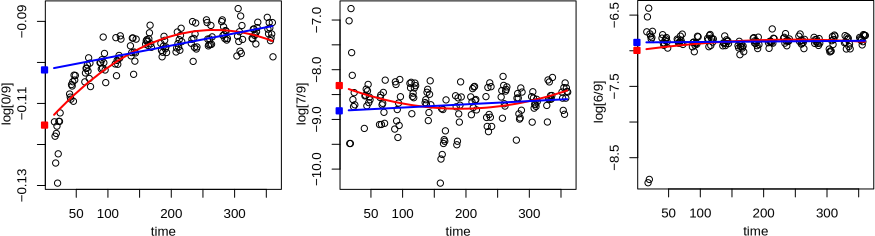
\includegraphics[width=\textwidth]{polyVSlin.pdf}
  \caption{Time-resolved mass spectrometry signals of the first
    aliquot of S-228 F2 sanidine, shown as blank-corrected log-ratios.
    The blue lines mark a linear fit to all data points after 50
    seconds.  The red lines show a polynomial to all the data (from 0
    seconds onwards).}
  \label{fig:polyVSlin}
\end{figure}

Figure~\ref{fig:polyVSlin} shows two model fits to the time-resolved
data of the first sample. A polynomial fit uses all the data and is
shown in red, whereas a linear fit uses only the data after 50 seconds
and is shown in blue. Which of these two time zero intercepts
correctly reflects the argon composition of the sample? The difference
between these methods results in up to a 14ka age difference. This
corresponds to an effect of 2.5\%, which is much greater than the
analytical precision (Table~\ref{tab:results}).  In my view this
accuracy issue needs to be resolved before we can discuss the
precision.\\

The age uncertainties are moderelately correlated with each other,
with correlation coefficients up to 0.5. This is shown graphically for
the linear regression model in Figure~\ref{fig:ellipses}. The
uncertainties and correlations can be broken down into components, but
before doing so it would be good to decide on a clearly justifiable
time zero regression strategy.

\begin{table}[!ht]
  \centering
  \captionsetup{width=11cm}
  \begin{tabular}{ccc|cc|cc}
    \# & t[WiscAr] & s.e.[t] &
    t[\texttt{Redux},lin.] & s.e.[t] &
    t[\texttt{Redux},poly.] & s.e.[t] \\ \hline
    1 & 514.79 & 4.24 & 513.08 & 3.07 & 514.05 & 7.75 \\
    2 & 516.98 & 2.79 & 529.62 & 1.97 & 515.78 & 3.43 \\
    3 & 509.60 & 2.47 & 512.85 & 1.95 & 505.42 & 3.27 \\
    4 & 509.89 & 2.75 & 517.14 & 2.61 & 501.72 & 4.70
  \end{tabular}
  \caption{\textsuperscript{40}Ar/\textsuperscript{39}Ar ages (in ka)
    and standard errors for S-228 F2 sanidine, comparing the results
    shown in the WiscAr spreadsheet with two \texttt{Ar-Ar\_Redux}
    calculations, one for the linear fit and one for the polynomial
    fit.}
  \label{tab:results}
\end{table}

\begin{figure}[!ht]
  \centering
  \captionsetup{width=10cm}
  \includegraphics[width=10cm]{ellipses.pdf}
  \caption{\textsuperscript{40}Ar/\textsuperscript{39}Ar results for
    four aliquots of S-228 F2 sanidine, using the linear fit.
    Uncertainties are shown as 95\% confidence ellipses. Error
    correlations fall between 0.21 (aliquots 1 and 4) and 0.50
    (aliquots 3 and 4).}
  \label{fig:ellipses}
\end{figure}

\bibliographystyle{/home/pvermees/Dropbox/abbrvplainnat}
\bibliography{/home/pvermees/Dropbox/biblio}

\end{document}
